\documentclass[spanish]{theme/pclreport}
\usepackage[utf8]{inputenc}
\usepackage[spanish]{babel}
\usepackage{float}
\usepackage{subcaption}
\usepackage{cite}
\usepackage{listings}
\usepackage{graphicx}
\usepackage{gensymb}


%\lstset { %
%    language=PHP,
%    backgroundcolor=\color{black!5}, % set backgroundcolor
%    basicstyle=\footnotesize,% basic font setting
%    commentstyle=\color{green},
%}

\definecolor{dkgreen}{rgb}{0,.6,0}
\definecolor{dkblue}{rgb}{0,0,.6}
\definecolor{dkyellow}{cmyk}{0,0,.8,.3}

\lstset{
  language        = php,
  backgroundcolor=\color{black!5},
  basicstyle      = \small\ttfamily,
  keywordstyle    = \color{dkblue},
  stringstyle     = \color{red},
  identifierstyle = \color{dkgreen},
  commentstyle    = \color{gray},
  emph            =[1]{php},
  emphstyle       =[1]\color{black},
  emph            =[2]{if,and,or,else},
  emphstyle       =[2]\color{dkyellow}}

\setlogo{PCL}
\pclsub{WorkShopDay}
\pcltitle{Programadores Chile}

\title{Workshop \\ Laravel 5.4 }
\author{
\begin{figure}[H]
	\centering
	
\includegraphics[scale=.2]{imagenes/laravel-logo.png}
\end{figure}}
	
\profesor{Expositor \\ Sebastian Zamorano Jara}

\date{25 de Marzo de 2017}



\begin{document}
\maketitle

\newpage

\vspace*{\fill}
\section*{Revisiones}
\begin{table}[H]
\centering
\begin{tabular}{cccc}
\textbf{Editor}   &                 \textbf{Comentarios}                       & \textbf{Versión} & \textbf{Fecha}  \\
Arturo Mantinetti & Diseño Template, estructura inicial y algunos apuntes      & 1.0              & 03/04/2017      \\
                  &                                                            &                  &                 \\
                  &                                                            &                  &                               
\end{tabular}
\end{table}
\vspace*{\fill}


\thispagestyle{empty} 

\tableofcontents



\chapter{Introducción}


\section{Resumen}




\chapter{Lo Nuevo en PHP 7}

\begin{itemize}  
\item Permite forzar tipos de entrada y salida de una función
\item Implementación del comparador $<=>$ retornando -1 0 1 según sea menor, igual o mayor
\item Nuevo Operador ?? Ver Listing 2.1
\end{itemize}


\begin{lstlisting}[caption={isset vs ??},captionpos=b]

<?php
// obtener el valor de $_GET['usuario'] y devolver 'nadie'
// si no existe.
$nombre_usuario = $_GET['usuario'] ?? 'nadie';
// Esto equivale a:
$nombre_usuario = isset($_GET['usuario']) ? $_GET['usuario'] : 'nadie';
\end{lstlisting}


\chapter{Aprendamos PHP Correctamente}

\section{Buenas Practicas en PHP}

\begin{itemize}  
\item Nunca usar echo
\
\end{itemize}





\chapter{Conozcamos Laravel}

\section{¿Por que Utilizarlo?}

La principal razón que se utiliza Laravel en el mercado es su facilidad de uso en comparado a otros frameworks. Ademas este tiene una gran comunidad en aumento. En el caso que debamos desarrollar una API, existe una version ligera conocida como Lumen.

\section{Estructura de Carpetas}

\subsection{.env}
Archivo de configuración de Laravel, este se encuentra en la carpeta principal, en este encontraremos las principales configuraciones de la base de datos, del correo electrónico que utilizara laravel y si se encuentra en modo de prueba.


\subsection{app}
En esta carpeta encontraremos los modelos, siendo estos las clases definidas por nosotros como entidades. \\
Dentro de app podemos encontrar la carpeta Console que contiene el archivo Kernel donde definiremos nuestros comandos protegidos de consola y el listado de acciones programadas.\\
También podemos encontrar la carpeta Controllers dentro de Http, en esta carpeta se sitúan los controladores de la aplicación, es decir donde añadiremos las lineas de código para procesar los datos que necesitamos, el nombre de los controladores por norma debe terminar en ``Controller.php''. \\ Dentro de Http encontraremos además una carpeta Middleware, acá van las funciones que nos permitirán filtrar peticiones y agregar distintas condiciones a estas. \\

\subsection{config}
Acá se encuentran los archivos de configuración, dentro del el archivo app.php podemos configurar el nombre de nuestra aplicación, la zona horaria, el lenguaje, cifrado y los paquetes que utilizaremos dentro de nuestra aplicación. También podremos encontrar archivos de configuración de correo, almacenamiento de archivos, cache, entre otros.

\subsection{database}
Nos centraremos en una carpeta migrations, que esta contenida dentro de esta. En este lugar encontraremos nuestros archivos de creación de la base de datos.

\subsection{public}
Esta carpeta es a la cual accederá el usuario via el navegador, aca el index es el encargado de importar el framework, también podremos agregar dentro de esta carpeta archivos css, js, imagenes, etc. que nosotros queramos que cualquiera tenga acceso sin filtro alguno.

\subsection{resources}
Dentro de esta carpeta encontraremos otra llamada views, acá es donde dejaremos todas las vistas en formato blade.php de nuestra aplicación. También podemos encontrar una carpeta llamada lang, en esta debemos agregar los lenguajes de Laravel que descarguemos.

\subsection{routes}
Acá encontraremos un archivo llamado web.php, este contiene las rutas de la aplicación, y en console.php tenemos la posibilidad de agregar nuestros propios comandos.

\subsection{storage}
Dentro de esta carpeta se almacenaran los archivos que subamos desde Laravel, también podremos encontrar el Log de el framework.







\chapter{Utilicemos Laravel}

\subsection{Instalando Laravel}
Para utilizar Laravel necesitamos tener previamente instalado php y composer, este ultimo lo podemos instalar del la siguiente forma:

\subsubsection{Composer en Windows}
Instalar composer en windows es una tarea simple, tan solo debemos descargar el instalador de \newline
 \textit{https://getcomposer.org/download/} y ejecutar el exe.
 
\subsubsection{Composer en Linux y OSX}
Debemos descargar el instalador de \textit{https://getcomposer.org/installer} y luego de esto lo ejecutamos con
\textit{\$ sudo php -- --install-dir=/usr/local/bin --filename=composer}  \newline

Luego de esto podremos crear nuestro proyecto con \newline \textit{composer create-project --prefer-dist laravel/laravel \textless nombre del proyecto\textgreater}

\subsection{Diagrama Funcionamiento}

\begin{figure}[H]
	\centering
	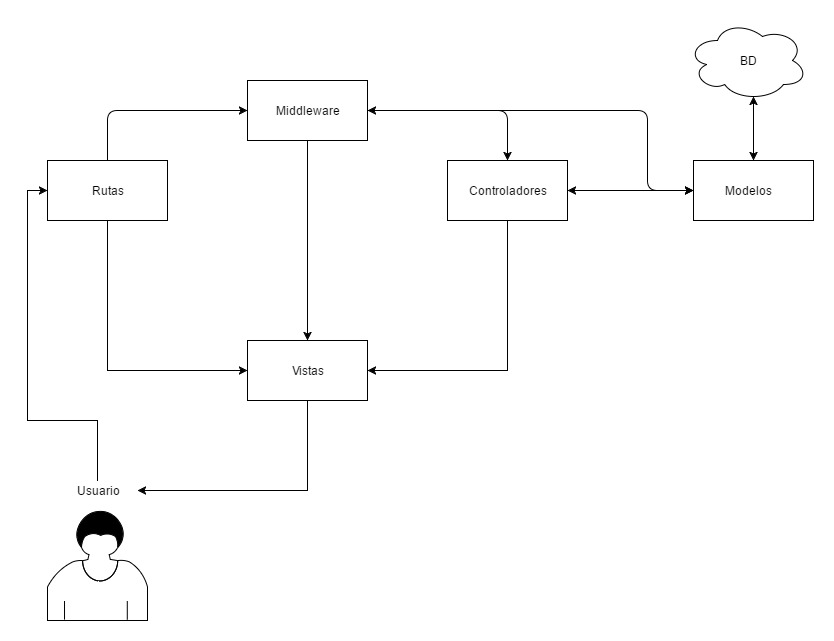
\includegraphics[scale=.4]{imagenes/diagrama.jpg}
	\caption{Diagrama Funcionamiento Laravel}
\end{figure}


\subsection{Modelos}
En laravel tenemos acceso a un ORM\footnote{(Object-Relational mapping, Mapeo Objeto-Relacional en español} llamado Eloquent, este hace uso de los Modelos como intermediarios o representantes de la base de datos, estos tienen la capacidad de detectar automáticamente la tabla si es que el nombre del modelo esta en singular y la tabla esta el mismo en plural. Dentro de estos modelos encontraremos y podremos usar una propiedad llamada fillable, donde los valores que se encuentren en esta propiedad parasan a ser un tipo de constructor, ya que podremos asignarlos en conjunto vía un arreglo y nos devolvera un nuevo objeto, con estos atributos. Tambien aca podremos relacionar objetos usando hasOne, hasMany, belongsTo y belongsToMany, es decir tiene uno, tiene muchos, pertenece a uno y pertenece a muchos. \newline

\begin{lstlisting}[caption={Ejemplo de Relaciones},captionpos=b]

//si tenemos un usuario que tiene libros lo podemos definir de la siguiente forma
public function libros()
{
    return $this->belongsTo('App\Libros', 'foreign_key', 'local_key');
}
\end{lstlisting}

Podemos crear la base de un modelo rápidamente gracias a artisan, para esto en la consola dentro del directorio raíz del proyecto escribimos $php$ $artisan$ $make:model$ $nombre-del-modelo$

\subsection{Controladores}
Acá es donde definiremos las peticiones y las manipularemos según lo que requiramos. Estos por convención debe contener Controller al final de su nombre. \newline 
Para crear un controlador lo hacemos vía consola con: \newline 
$php$ $artisan$ $make:controller$ $nombre-del-controlador$

\subsection{web.php}
En este archivo se encuentran las rutas, estas las definiremos de la siguiente forma:

\begin{lstlisting}[caption={Ejemplo de rutas},captionpos=b]

Route::get('/enlace', 'NombreControladorr@Funcion');
Route::post('/insertar', 'NombreControlador@Funcion');
\end{lstlisting}

\subsection{Creando Autenticación de Usuarios}
En laravel podemos crear de una forma muy simple un sistema de usuarios con el siguiente comando: \newline
$php$ $artisan$ $make:auth$ \newline
Esto nos generara las vistas de ingresar, registrarse y recuperar contraseña, el modelo de usuario, mas sus respectivos controladores.



\listoffigures


\end{document}
